\documentclass[11pt, a4paper]{article}

% --- Essential Packages ---
\usepackage[utf8]{inputenc}    % Text encoding
\usepackage{graphicx}          % Required for inserting images
\usepackage{url}               % Required for robust URL handling
\usepackage{hyperref}          % Required for links and URLs
\usepackage{geometry}          % Adjust page margins
\geometry{margin=2.5cm}

% --- Document Information ---
\title{\textbf{Labwork 2 Report: Get to know your machine}}
\author{Lucien Elyas Bedrane \\ Student ID: 2640012}
\date{\today}

\begin{document}

\maketitle

% --- Section 1: Objective Breakdown ---
\section{Objectives \& Breakdown}
In this lab, we want to explore the Python Numba basic functions to recover basic information regarding our GPU.

% --- Section 2: Code Output Image ---
\section{Code Execution \& Results}
Below is the screenshot demonstrating the execution and final output of the code:

\begin{figure}[h!]
    \centering
    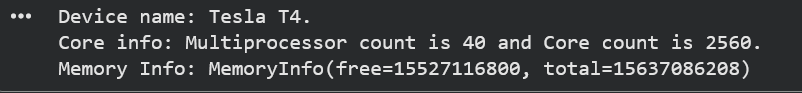
\includegraphics[width=0.8\textwidth]{script_output} 
    \caption{Screenshot of the program's output.}
    \label{fig:code_output}
\end{figure}

% --- Section 3: Sources ---
\section{Sources \& References}
The following resources and documentation were used to complete this work:

\begin{itemize}
    \item Numba CUDA Host API Documentation: \\
    \url{https://numba.readthedocs.io/en/stable/cuda-reference/host.html#device-management}
    
    \item Stack Overflow guide that allowed me to get the numbers of cores and the multiprocessor count: \\
    \url{https://stackoverflow.com/questions/63823395/how-can-i-get-the-number-of-cuda-cores-in-my-gpu-using-python-and-numba/63833950#63833950}
\end{itemize}

\end{document}
